 \section{Логистическая регрессия}
 
 \subsection{Задача}
 
 В прошлой <<главе>> мы научились решать задачи \textit{регрессии} с помощью \textit{линейной регресии}. Возникает очевидный вопрос: как же тогда решать задачу \textit{классификации}? Попробуем обобщить модель \textit{линейной регрессии} на \textit{классификацию}.
 
 \subsection{Модель}
 Давайте, для начала, рассмотрим задачу \textit{бинарной классификации}.
 
 Что будет, если мы просто предскажем 0 или 1 с помощью \textit{линейной регрессии}? Скажем, что значения, большие 0.5 относятся к \textit{первому классу}, меньшие - к \textit{второму} классу.
 
При таком подходе модель никак не учитывает свою \textit{<<уверенность>>} в ответе. Мы не увидим отличие, между значением, равным 0.5 и равным 1000. Хотелось бы научиться получать \textbf{вероятность принадлежности к классу 1}.

Давайте преобразовывать ответ модели, который находится в интервале $(-\infty;+\infty)$ в ответ из интервала $(0; 1)$. Такие преобразования называются \textbf{сигмоидами}.

\begin{center}
    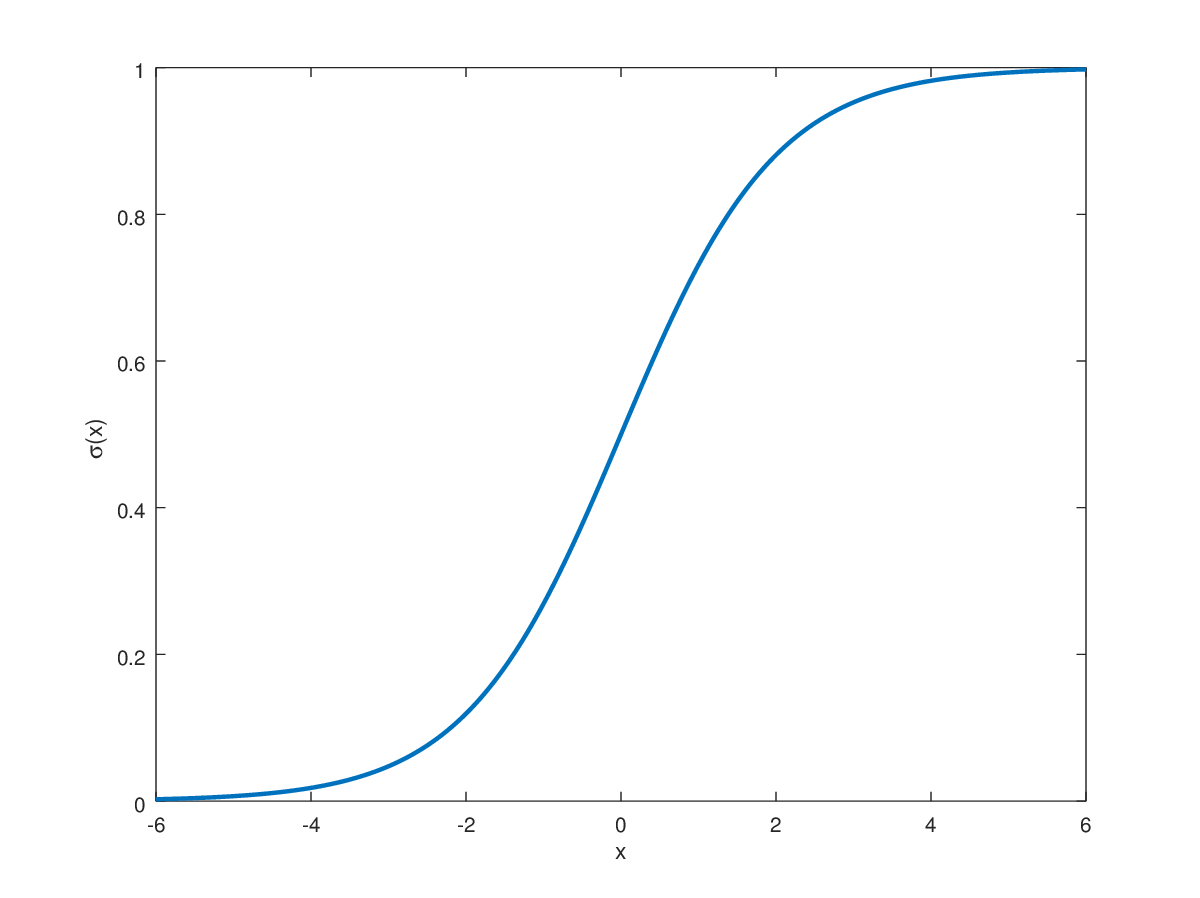
\includegraphics[scale=0.65]{tickets/pictures/sigmoid_function.png}
\end{center}

Обычно используют сигмоиду $\sigma(y) = \frac{1}{1 + e^{-y}}$.

\subsection{Функция потерь}

Так как у нашей модели изменились ответы, нам необходимо поменять функцию ошибки. Давайте посмотрим на предсказания модели и вычислим вероятность того, что модель <<угадает>> классы для всех объектов.

$$P_{all} = \prod_{i | y_i=1}p_i \prod_{i | y_i=0}(1 - p_i)$$

Нам необходимо максимизировать эту вероятность.

Работать с произведением неудобно, поэтому возьмем логарифм.

$$\ln{P_{all}} = \sum_{i | y_i=1}\ln{p_i} + \sum_{i | y_i=0}\ln(1 - p_i)$$

Если взять данное значение с отрицанием, получится наша новая функция потерь - \textbf{Logloss}.

$$Logloss = -\ln{P_{all}} = -\sum_{i | y_i=1}\ln{p_i} - \sum_{i | y_i=0}\ln(1 - p_i)$$

Описанный алгоритм называется \textbf{Логистическая регрессия} и служит для бинарной классификации.

\subsection{Мультиклассовая классификация}
Если мы имеем задачу мультиклассовой классификации с \textbf{n} классами, давайте обучим $n$ логистических регрессий, в $i$-й логистической регресии будем предсказывать вероятность, что объект относится к классу $i$. 

Как ответ можно взять класс с максимальной вероятностью.